\documentclass{article}

\usepackage{tikz-feynman}

\begin{document}

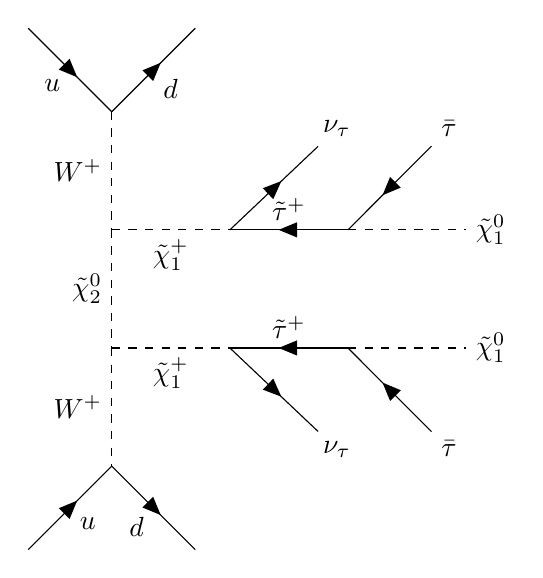
\begin{tikzpicture}
	\begin{feynman}
		\vertex (a);
		\vertex [below right=of a] (b);
		\vertex [above right=of b] (c);
		\vertex [below=of b] (d);
		\vertex [below=of d] (e);
		\vertex [below=of e] (f);
		\vertex [below left=of f] (g);
		\vertex [below right=of f] (h);
		\vertex [right=of d] (i);
		\vertex [right=of i] (l);
		\vertex [right=of l] (m){\(\tilde{\chi}^{0}_{1}\)};
		\vertex [above right=of i] (n){\(\nu_{\tau}\)};
		\vertex [above right=of l] (o){\(\bar{\tau}\)};
		\vertex [right=of e] (p);
		\vertex [right=of p] (q);
		\vertex [right=of q] (r){\(\tilde{\chi}^{0}_{1}\)};
		\vertex [below right=of p] (s){\(\nu_{\tau}\)};
		\vertex [below right=of q] (t){\(\bar{\tau}\)};




		\diagram* {
			(a) -- [fermion, edge label'=\(u\)] (b) -- [fermion, edge label'=\(d\)] (c);
			(b) -- [scalar, edge label'=\(W^{+}\)] (d) -- [scalar, edge label'=\(\tilde{\chi}^{0}_{2}\)](e) -- [scalar, edge label'=\(W^{+}\)](f);
			(g) -- [fermion, edge label'=\(u\)] (f) -- [fermion, edge label'=\(d\)] (h); 
			(o) -- [fermion] (l) -- [fermion, edge label'=\(\tilde{\tau}^{+}\)] (i) -- [fermion] (n);
			(d) -- [scalar, edge label'=\(\tilde{\chi}^{+}_{1}\)] (i);
			(l) -- [scalar] (m);
			(t) -- [fermion] (q) -- [fermion, edge label'=\(\tilde{\tau}^{+}\)] (p) -- [fermion] (s);
			(e) -- [scalar, edge label'=\(\tilde{\chi}^{+}_{1}\)] (p);
			(q) -- [scalar] (r);
		};

	\end{feynman}

\end{tikzpicture}

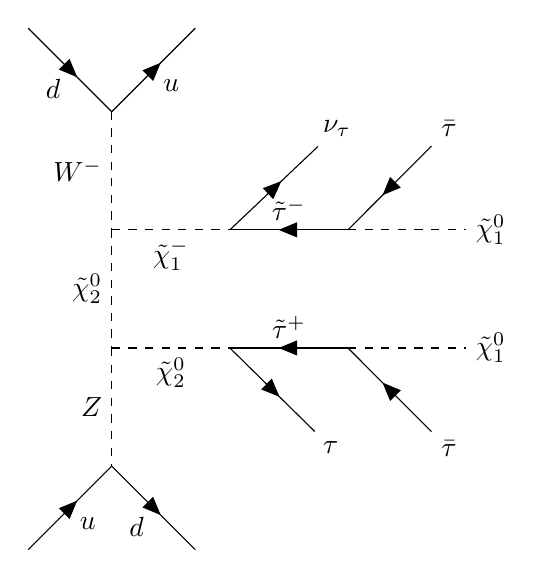
\begin{tikzpicture}
	\begin{feynman}
		\vertex (a);
		\vertex [below right=of a] (b);
		\vertex [above right=of b] (c);
		\vertex [below=of b] (d);
		\vertex [below=of d] (e);
		\vertex [below=of e] (f);
		\vertex [below left=of f] (g);
		\vertex [below right=of f] (h);
		\vertex [right=of d] (i);
		\vertex [right=of i] (l);
		\vertex [right=of l] (m){\(\tilde{\chi}^{0}_{1}\)};
		\vertex [above right=of i] (n){\(\nu_{\tau}\)};
		\vertex [above right=of l] (o){\(\bar{\tau}\)};
		\vertex [right=of e] (p);
		\vertex [right=of p] (q);
		\vertex [right=of q] (r){\(\tilde{\chi}^{0}_{1}\)};
		\vertex [below right=of p] (s){\(\tau\)};
		\vertex [below right=of q] (t){\(\bar{\tau}\)};




		\diagram* {
			(a) -- [fermion, edge label'=\(d\)] (b) -- [fermion, edge label'=\(u\)] (c);
			(b) -- [scalar, edge label'=\(W^{-}\)] (d) -- [scalar, edge label'=\(\tilde{\chi}^{0}_{2}\)](e) -- [scalar, edge label'=\(Z\)](f);
			(g) -- [fermion, edge label'=\(u\)] (f) -- [fermion, edge label'=\(d\)] (h); 
			(o) -- [fermion] (l) -- [fermion, edge label'=\(\tilde{\tau}^{-}\)] (i) -- [fermion] (n);
			(d) -- [scalar, edge label'=\(\tilde{\chi}^{-}_{1}\)] (i);
			(l) -- [scalar] (m);
			(t) -- [fermion] (q) -- [fermion, edge label'=\(\tilde{\tau}^{+}\)] (p) -- [fermion] (s);
			(e) -- [scalar, edge label'=\(\tilde{\chi}^{0}_{2}\)] (p);
			(q) -- [scalar] (r);
		};

	\end{feynman}

\end{tikzpicture}

\end{document}
